\documentclass[a4paper,11pt]{article}

% Francais
%\usepackage[francais]{babel}
\usepackage[utf8]{inputenc} %for accentuated letters
\usepackage[T1]{fontenc}  %important for correct cesure of accentuated letter
%\usepackage{ae,aecompl,aeguill}   %important for fonts in pdf
\usepackage{ae,aecompl}   %important for fonts in pdf

%For comments
\usepackage{verbatim} 
\usepackage{url}

%Graphics
\usepackage{graphicx}% Include figure files
\usepackage{dcolumn}% Align table columns on decimal point
\usepackage{rotating}
\usepackage{epstopdf}%automatic ps -> pdf conversion
\usepackage{tikz}
\usepackage{tikz-qtree}

%Maths
\usepackage{amstext,amsmath,amssymb,amsfonts}
\usepackage{bm}% bold math

% Fonts
%\usepackage{txfonts}
%\usepackage{bbm}
%\usepackage[cspex,bbgreekl]{mathbbol}

% Different font in captions
\newcommand{\captionfonts}{\small}
\makeatletter  % Allow the use of @ in command names
\long\def\@makecaption#1#2{%
  \vskip\abovecaptionskip
  \sbox\@tempboxa{{\captionfonts #1: #2}}%
  \ifdim \wd\@tempboxa >\hsize
    {\captionfonts #1: #2\par}
  \else
    \hbox to\hsize{\hfil\box\@tempboxa\hfil}%
  \fi
  \vskip\belowcaptionskip}
\makeatother   % Cancel the effect of \makeatletter

% References
\usepackage{cite} %to group multipled references
\usepackage[hidelinks]{hyperref}

%--------------------------------------

% Colors
\usepackage{color}
\definecolor{lightblue}{rgb}{0.2,0.2,0.7}
\definecolor{darkblue}{rgb}{0,0.25,0.5}
\definecolor{redbrown}{rgb}{0.875,0.25,0.125}
\definecolor{darkgreen}{rgb}{0,0.5,0}

%Newcommands
\renewcommand{\b}[1]{\textbf{#1}}
\renewcommand{\l}[1]{\hyperlink{#1}{\textbf{#1}}}
\renewcommand{\t}[1]{\hypertarget{#1}{\textbf{#1}}}

%Headers
\usepackage{fancyhdr}

%Margins
\setlength{\topmargin}{-1cm}     %top margin
\setlength{\textheight}{24cm}    %bottom margin
\setlength{\textwidth}{16cm}     %right margin
\setlength{\oddsidemargin}{0cm}  %left margin (for odd pages or single sided)
\setlength{\evensidemargin}{0cm} %left margin (for even pages if using twoside)

% paragraph with newline
\makeatletter
\renewcommand\paragraph{\@startsection{paragraph}{4}{\z@}%
  {-3.25ex\@plus -1ex \@minus -.2ex}%
  {1.5ex \@plus .2ex}%
  {\normalfont\normalsize\bfseries}}
\makeatother

\usepackage{xstring}
\newcommand{\makesub}[1]{%
  \saveexpandmode\noexpandarg
  \StrSubstitute{#1}{\_}{_}[\temp]%
  \restoreexpandmode
}
\newcommand\see[1]{
  \makesub{#1}
  [see: \hyperref[entry:\temp]{#1}]
}
\newcommand\entry[2]{
  \saveexpandmode\noexpandarg
  \vspace*{.5em}
  \IfBeginWith{#1}{[}{
    \IfSubStr{#1}{(}{
      \StrBetween{#1}{] }{(}[\temp]
    }{
      \StrBehind{#1}{] }[\temp]
    }
  }{
    \IfSubStr{#1}{(}{
      \StrBefore{#1}{(}[\temp]
    }{
      \StrSubstitute{#1}{\_}{_}[\temp]
    }
  }
  \noindent\underline{\textbf{\temp}} (usage: {\tt #1})
  \label{entry:\temp}\addcontentsline{toc}{paragraph}{\temp}
  \restoreexpandmode

  \vspace*{.5em}
  \noindent\begin{tabular}{m{.001\linewidth}m{.999\linewidth}}
    & {#2}
  \end{tabular}
}

\usepackage{amsfonts}
\usepackage{amsmath}
\usepackage{physics}

\usepackage[english]{babel}
\usepackage{underscore}

\begin{document}

\title{Notes on the programming style in CHAMP}

%%%%%%%%%%%%%%%%%%%%%%%%%%%%%%%%%%%%%%%%%%%%%%%%%%%%%%%%%%%%%%%%%%%%%%%%%%%%%
\author{Julien Toulouse\\
Laboratoire de Chimie Th\'eorique\\Universit\'e Pierre et Marie Curie et CNRS, 75005 Paris, France\\
julien.toulouse@upmc.fr}

%%%%%%%%%%%%%%%%%%%%%%%%%%%%%%%%%%%%%%%%%%%%%%%%%%%%%%%%%%%%%%%%%%%%%%%%%%%%%
\date{\today}

\maketitle

\setcounter{secnumdepth}{5}
\setcounter{tocdepth}{5}

\tableofcontents

\vspace*{5em}

These notes describe the programming paradigm used in the Fortran 90 files of the program CHAMP. This programming paradigm was invented by the theoretical chemist and legendary programmer François Colonna and was given different names over the years:
Open Structured Interfaceable Programming Environment (OSIPE)~\cite{ColJolPoiAngJan-CPC-94},
Deductive Object Programming~\cite{Col-ARX-06},
Implicit Reference to Parameters (IRP)~\cite{Sce-ARX-09},
as well as Minimal Explicit Declaration (MED).
Even though we describe a Fortran implementation of it, this programming paradigm is not restricted to any particular programming language, and in fact has been implemented in many languages. The particular Fortran implementation that I made in CHAMP was very much inspired by the implementation in the program QMCMOL~\cite{Qmc-PROG-XX} mainly made by Roland Assaraf.

\section{Introduction}
A Fortran computer program produces {\it objects}, which are Fortran variables, of any type or dimension (scalar/array), containing quantities that we are after. For example, {\tt psi} may be an object containing the value of a wave function evaluated at some electron coordinates. This object {\tt psi} is constructed from other objects. For example, for the case of a Jastrow $\times$ single determinant wave function, we have {\tt psi = jastrow * determinant} where {\tt jastrow} and {\tt determinant} are the values of the Jastrow factor and of the Slater determinant at the same electron coordinates. The later objects are themselves constructed from yet other objects. For example, {\tt determinant} may be constructed from {\tt orbitals} which is an array containing the values of the orbitals at the considered electron coordinates. And so on.

Clearly, there are {\it dependencies} between these objects, in the sense that the construction of a given object requires that other objects have already been constructed. In other words, the order in which the objects are constructed is important. Usually, in Fortran programs, these dependencies are {\it not} made explicit, and making sure that the order of the construction of the objects is correct is left to the programmer. In large codes, this may make difficult the implementation of a new object.

In the programming paradigm used here, the dependencies between the objects are made explicit. The programmer then does not need to take care of the order of construction of the objects. This facilitates the implementation of new objects.

\section{Basis of the paradigm and implementation}

The programming paradigm is best explained on a simple example. 

\subsection{Dependency tree and building subroutines}

Consider again the object {\tt psi}, constructed from two objects {\tt jastrow} and {\tt determinant}, themselves constructed from other objects according to the following {\it dependency tree}:


\begin{center}
\begin{tikzpicture}
\Tree [.\node[draw]{\tt psi};
  [.\node[draw]{\tt jastrow};     
    [.{\tt jastrow_parameters} ]
    [ [ [ .\node(coord){\tt electron_coordinates}; ] ] ] ]
  [.\node[draw]{\tt determinant}; 
    [.\node[draw]{\tt orbitals};
      [.\node[draw](basis){\tt basis_functions}; [ {\tt basis_parameters} ] ] [.{\tt coefficients}
      ] ] ] ]
\draw (coord)--(basis);
\end{tikzpicture}
\end{center}

Note that, strictly speaking, this is not a tree but a graph since the branches are not necessarily disjoint. For example, in the example above, the object {\tt electron_coordinates} connects the two branches. We will nevertheless use the vocabulary of computer trees.

This tree encodes the dependencies between the objects. For example, {\tt psi} depends on both {\tt jastrow} and {\tt determinant}. In turn, {\tt jastrow} depends on {\tt jastrow_parameters} and {\tt electron_coordinates}. And so on. We will say that {\tt psi} is a {\it child} of {\tt jastrow} and {\tt determinant}, and {\tt jastrow} and {\tt determinant} are the {\it parents} of  {\tt psi}. The objects without any parents (those that are not boxed: {\tt jastrow_parameters}, {\tt electron_coordinates}, {\tt basis_parameters}, {\tt coefficients}) are the {\it leaves} of the tree. These generally correspond to input parameters which must be given by the user when running a calculation.

\vspace{1em}
The practical implementation of the dependency tree in the program is explained in the next section. For the moment, let us describe how calculations are done, assuming that the information about the dependency tree is available in the program.
Each object which is not a leaf of the tree has a {\it building subroutine} which constructs it. So, written schematically, we have the five following building subroutines in the program, corresponding to the five boxed objects of the tree:

\vspace{0.5cm}
\noindent
{\tt subroutine psi_bld\\
psi = jastrow * determinant\\
end subroutine psi_bld}

\vspace{0.5cm}
\noindent
{\tt subroutine jastrow_bld\\
jastrow  = $f(${\tt jastrow_parameters}$,${\tt electron_coordinates}$)$\\
end subroutine jastrow_bld}

\vspace{0.5cm}
\noindent
{\tt subroutine determinant_bld\\
determinant  = $f(${\tt orbitals}$)$\\
end subroutine determinant_bld}

\vspace{0.5cm}
\noindent
{\tt subroutine orbitals_bld\\
orbitals  = $f(${\tt basis_functions}$,${\tt coefficients}$)$\\
end subroutine orbitals_bld}

\vspace{0.5cm}
\noindent
{\tt subroutine basis_functions_bld\\
basis_functions  = $f(${\tt electron_coordinates}$,${\tt basis_parameters}$)$\\
end subroutine basis_functions_bld}

\vspace{0.5cm}
\noindent
Here, to simplify, we have shown the explicit expression of {\tt psi} only, the expressions of the other objects are just written as (complicated) functions $f$.

\vspace{0.5cm}
The most part of the program is made of building subroutines, but they do {\it not} make {\it all} the program. Here are examples of subroutines which are {\it not} building subroutines:
\begin{itemize}
\item The subroutines reading the input. This is usually where the leaf objects are created.
\item The subroutines writing the output.
\item The subroutines containing the main iterative algorithms, such as the Monte Carlo algorithm or the wave-function optimization algorithm.
\end{itemize}

\subsection{Implementation of the dependency tree (object_create and object_needed)}

In CHAMP, it was chosen to give the data of the dependencies between the objects directly in the building subroutines. The advantage of this is that all the information about a given object is localized in its building subroutine, and not delocalized in different places in the code.

Hence, each building subroutine contains a {\it header} part where the object created by this building subroutine is indicated by {\tt call object_create(`...')} and all the parent objects are listed by {\tt call object_needed(`...')}. Thus, the building subroutines of our simple example actually look like:

\vspace{0.5cm}
\noindent
{\tt subroutine psi_bld\\
if(header) then\\
\phantom{xx} call object_create(`psi')\\
\phantom{xx} call object_needed(`jastrow')\\
\phantom{xx} call object_needed(`determinant')\\
\phantom{xx} return\\
endif\\
psi = jastrow * determinant\\
end subroutine psi_bld}

\vspace{0.5cm}
\noindent
{\tt subroutine jastrow_bld\\
if(header) then\\
\phantom{xx} call object_create(`jastrow')\\
\phantom{xx} call object_needed(`jastrow_parameters')\\
\phantom{xx} call object_needed(`electron_coordinates')\\
\phantom{xx} return\\
endif\\
jastrow  = $f(${\tt jastrow_parameters}$,${\tt electron_coordinates}$)$\\
end subroutine jastrow_bld}

\vspace{0.5cm}
\noindent
{\tt subroutine determinant_bld\\
if(header) then\\
\phantom{xx} call object_create(`determinant')\\
\phantom{xx} call object_needed(`orbitals')\\
\phantom{xx} return\\
endif\\
determinant  = $f(${\tt orbitals}$)$\\
end subroutine determinant_bld}

\vspace{0.5cm}
\noindent
{\tt subroutine orbitals_bld\\
if(header) then\\
\phantom{xx} call object_create(`orbitals')\\
\phantom{xx} call object_needed(`basis_functions')\\
\phantom{xx} call object_needed(`coefficients')\\
\phantom{xx} return\\
endif\\
orbitals  = $f(${\tt basis_functions}$,${\tt coefficients}$)$\\
end subroutine orbitals_bld}

\vspace{0.5cm}
\noindent
{\tt subroutine basis_functions_bld\\
if(header) then\\
\phantom{xx} call object_create(`basis_functions')\\
\phantom{xx} call object_needed(`electron_coordinates')\\
\phantom{xx} call object_needed(`basis_parameters')\\
\phantom{xx} return\\
endif\\
basis_functions  = $f(${\tt electron_coordinates}$,${\tt basis_parameters}$)$\\
end subroutine basis_functions_bld}

\vspace{0.5cm}
For all the building subroutines, the header part is executed only once at the beginning of the execution of the program in order to construct the dependency tree. Then, in the actual calculations we always have {\tt header=.false.} so the header part is bypassed.

\subsection{Manipulating objects (object_provide and object_modified)}

%\subsection{call object\_provide}

All subroutines can manipulate the objects of the dependency tree with the two main commands explained here: {\tt call object_provide} and {\tt call object_modified}.

For example, suppose that the programmer wants to print out the value of {\tt psi} at some place in the code (outside the building subroutines). He just needs to write the following lines:

\vspace{0.5cm}
\noindent
{\tt call object_provide(`psi')\\
write(6,*) `psi=',psi}

\vspace{0.5cm}
The instruction {\tt call object_provide(`psi')} does the following:\\
It checks if the object {\tt psi} is {\it valid}, i.e. if it has already been calculated and can be used.
\begin{itemize}
\item If yes, then nothing is done. 
\item If no, then the program checks if its parents {\tt jastrow} and {\tt determinant} are valid. 
\begin{itemize}
\item If both are valid, then the program calls the building subroutine {\tt psi_bld} and marks {\tt psi} as valid.
\item If, for instance, only {\tt determinant} is not valid, then the program checks if its parent {\tt orbitals} is valid. If {\tt orbitals} is valid, then the program calls the building subroutine {\tt determinant_bld}, marks {\tt determinant} as valid, then calls the building subroutine {\tt psi_bld} and marks {\tt psi} as valid. If {\tt orbitals} is not valid, the programs checks its parents, and so on.
\end{itemize}
\end{itemize}
In other words, {\tt object_provide(`psi')} goes down recursively the dependency tree under {\tt psi} until it finds valid objects. It then climbs up the dependency tree, constructing the objects one after the other, in the correct order, until it finally constructs {\tt psi}.

In the case where {\tt object_provide(`psi')} goes down to a leaf object of the dependency tree (for example, {\tt basis_parameters}) which is {\it not} valid, then it gives an error message indicating that this leaf object is necessary to construct {\tt psi} but does not know how to construct this leaf object. Indeed, since a leaf object does not have a building subroutine, the program does not know how to construct it. Leaf objects are instead usually read in from the input file at the beginning of execution and marked as valid then.

\vspace{0.5cm}
In summary, {\tt call object_provide(`psi')} has several advantages:
\begin{itemize}
\item It is {\it simple}. The programmer just needs to know the name of the object that he wants, here `psi'. He does not need to know how this object is calculated by the program. He does not need to know about intermediate objects such as {\tt orbitals}.
\item It is {\it safe}. If a necessary leaf object is not available, the program will properly stops and explains what is missing.
\item It is {\it efficient}, in the sense that this mechanism ensures that only what is needed is calculated, nothing more.
\end{itemize}

%\subsection{call object\_modified}
Another important ingredient remains to be explained. What if the value of an object, say {\tt electron_coordinates}, is modified? Then, we need to make sure that if we need any child or grandchild object of {\tt electron_coordinates}, this object must be recalculated with the new value of {\tt electron_coordinates}. This is done by inserting, just after modifying {\tt electron_coordinates}, the instruction {\tt call object_modified(`electron_coordinates')}:

\vspace{0.5cm}
\noindent
{\tt electron_coordinates = (-2.1, 0.7, 1.5)\\
call object_modified(`electron_coordinates')
}

\vspace{0.5cm}
The instruction {\tt call object_modified(`electron_coordinates')} marks {\tt electron_coordinates} as valid, and recursively climbs up the dependency tree to mark as {\it invalid} all the objects depending on {\tt electron_coordinates}, namely {\tt jastrow},  {\tt basis_functions}, {\tt orbitals}, {\tt determinant}, {\tt psi}. 

Thus, if any one of these objects is asked for afterwards, it will be recalculated with the new value of {\tt electron_coordinates}. This is a {\it safe} mechanism since it prevents the programmer from forgetting to update objects in an iterative algorithm, a frequent bug otherwise.

Note that a typical use of {\tt call object_modified} is after reading in leaf objects from the input to mark them as valid.

\section{Interface with the non-MED part}

The objects created in the non-MED files do not have building subroutines. If they are not available, the program does not know how to construct them. Nevertheless, to facilitate their use in the MED part, they can be added as leaf objects of the dependency tree. For this, we just need to add {\tt call object_modified(`...')}, for example in the line just after a non-MED object has been constructed. This provides a safe mechanism for using them, making sure that we use them only when they have been already calculated. In fact, I found this extremely useful when I started to program in CHAMP. 

When this is judged useful, a non-MED object can be converted to a MED object, i.e. we write a proper building subroutine for it and it is then a normal object of the dependency tree. The non-MED part of the code can then be progressively evolved in the style of the MED part.


\section{More details}

\subsection{A building subroutine can create more than one object}

Often, it is convenient to construct in the same building subroutine several objects. A given building subroutine thus generally creates several objects. For example, if the building subroutine {\tt jastrow_bld} creates the two object {\tt jastrow} and {\tt jastrow_gradient}, it will look like:

\vspace{0.5cm}
\noindent
{\tt subroutine jastrow_bld\\
if(header) then\\
\phantom{xx} call object_create(`jastrow')\\
\phantom{xx} call object_create(`jastrow_gradient')\\
\phantom{xx} call object_needed(`jastrow_parameters')\\
\phantom{xx} call object_needed(`electron_coordinates')\\
\phantom{xx} return\\
endif\\
jastrow  = $f(${\tt jastrow_parameters}$,${\tt electron_coordinates}$)$\\
jastrow_gradient  = $g(${\tt jastrow_parameters}$,${\tt electron_coordinates}$)$\\
end subroutine jastrow_bld}

\vspace{0.5cm}
With this extension, the nodes of the dependency tree are no longer the objects but instead the building subroutines, each one creating a list of objects. This extension does not cause any problem.

\subsection{Dynamic allocations inside the building subroutines}

If an object is an array, it is dynamically allocated inside its building subroutine, using {\tt call object_alloc}. For example:

\vspace{0.5cm}
\noindent
{\tt call object_alloc('orbitals', orbitals, norb)\\
do i=1,norb\\
\phantom{xx} orbitals(i) = ...\\
enddo}
\vspace{0.5cm}

Note that the dimension {\tt norb} itself is usually an object handled by the dependency tree. If it changes during the calculation, the array will be reallocated with the new size.

\subsection{Indexes of objects}
The functions {\tt object_modified(`...')} and {\tt object_provide(`...')} take as argument the name of an object given as a string. The name of the object is then looked up in an array which can take some time. If these functions are called in a part of the code that is very often executed, this is not efficient. In this case, we use directly the index of the object in the array, instead of its name. For example:

\vspace{0.5cm}
\noindent
{\tt call object_modified_by_index(electron_coordinates_index)}

\vspace{0.5cm}
\noindent
{\tt call object_provide_by_index(psi_index)}


\section{Programming Manual}

\subsection{What happens at the beginning of a run?}

\subsection{Definitions}

In Fortran, we cannot store the name of an object in a variable : once the code is compiled, the name is lost.
If we want to operate on dependencies, we need to retain the names, i.e. we need to have a mapping between each name and a variable.
In the CHAMP's implementation of the MED paradigm, there are Fortran objects, and they in general have a string {\tt `name'} and an integer {\tt `index'}.

Note that almost all basic MED instructions are given with the {\tt `name'} variable.
When a {\tt `name'} is given, the MED machinery searches for the corresponding {\tt `index'} ; in the core machinery, everything is done with the indexes.
Since the search can be costly, as stated before, for repetively used Fortran objects, it is possible to directly give the {\tt `index'}.

In the following sections, we give a glossary of basic and more advanced MED commands implemented in CHAMP.

\subsubsection{Types}

To well understand the commands described in the next sections, one first need to understand how informations about the objects and nodes are stored.

\entry{`object'}{
  The informations on an object are stored into a type {\tt object}.
  All the objects are accumulated in an array {\tt objects} of type {\tt object},
  and the object index is the position of an object in that array.
  The type {\tt object} contains:

  \vspace{.5em}
  \noindent\begin{tabular}{m{.26\linewidth}m{2mm}m{.37\linewidth}m{.33\linewidth}}
    {\tt character            }&::& {\tt name                           }& its name\\
    {\tt logical              }&::& {\tt associated                     }& is it associated?\\
    {\tt character            }&::& {\tt type                           }& its type\\
    {\tt integer, allocatable }&::& {\tt dimensions (:)                 }& its dimensions\\
    {\tt logical              }&::& {\tt walkers = .false.              }& \\
    {\tt logical              }&::& {\tt unweighted = .false.           }& \\
    {\tt logical              }&::& {\tt valid                          }& is it valid?\\
    {\tt logical              }&::& {\tt freezed = .false.              }& is it freezed?\\
    {\tt logical              }&::& {\tt object_depend_valid = .false.  }& \\
    {\tt integer              }&::& {\tt node_create_index = 0          }& its building routine\\
    {\tt integer, allocatable }&::& {\tt nodes_depend_index (:)         }& \\
    {\tt pointer              }&::& {\tt pointer_[type]                 }& \\
    {\tt logical              }&::& {\tt saved    = .false.             }& \\
    {\tt real                 }&::& {\tt save_[type]                    }& \\
    (and statistical stuff)    &::&
\end{tabular}
}

\entry{`node'}{
  The informations on a node (a building routine) are stored into a type {\tt node}.
  All the nodes are accumulated in an array {\tt nodes} of type {\tt node}.
  The type {\tt node} contains:

  \vspace{.5em}
  \begin{tabular}{m{.26\linewidth}m{2mm}m{.37\linewidth}m{.33\linewidth}}
    {\tt character            }&::& {\tt routine_name                  }& its name \\
    {\tt integer              }&::& {\tt routine_address               }& its address \\
    {\tt integer, allocatable }&::& {\tt objects_needed_index(:)       }& the list of needed objects \\
    {\tt integer, allocatable }&::& {\tt objects_create_index(:)       }& the list of created objects \\
    {\tt logical              }&::& {\tt valid                         }& is it valid? \\
    {\tt logical              }&::& {\tt debug = .false.               }&  \\
    {\tt logical              }&::& {\tt entered = .false.             }&  \\
    {\tt integer              }&::& {\tt calls_nb = 0                  }& stat data \\
    {\tt real                 }&::& {\tt cpu_duration = 0.d0           }& stat data \\
  \end{tabular}
}

\vspace{1em}
\noindent Hence, for example:

    {\tt nodes(objects(object_index)\%node_create_index)\%routine_name}

\noindent will give you the {\tt routine_name} of
the routine whose index is stored in {\tt node_create_index} of
the current object (known by its {\tt object_index}):
this is the name of the routine creating the object of index {\tt object_index} !


\subsubsection{Basics}

In this section, we describe in a glossary manner the basic commands of the MED implementation in CHAMP.
Those are the commands that are to be called when writting new code or modifying code.
In particular they can be found in all the files in CHAMP,
by contrast to the ``deeper machinery'' commands described in the next section,
that are (almost) only called in the ``{\tt MED_tools/*f90}'' files themselves.

\vspace{1em}

\entry{[sub] object_create(`name'[,\tt `index'])}{
  Catalogs an object known by its {\tt `name'}
  with the current building node index, 
  and possibly returns its (newly produced) {\tt `index'}.

  This uses {\tt object_add_once_and_index}.
  \vspace{1em}

  In details:
  \vspace{.5em}

  \begin{minipage}{\linewidth}\begin{itemize}
  \item register that the current node creates the object
  \\    ({\tt objects(index)\%node_create_index = node_current_index})
  \item and that the object is created by the current node
  \\    (add {\tt index} to {\tt nodes(node_current_index)\%objects_create_index})
  \end{itemize}\end{minipage}
}

\entry{[sub] object_needed(`name')}{
  Catalogs a dependency of the current building node.

  This uses {\tt object_add_once_and_index} (in case the object itself is not already catalogued).
  \vspace{1em}

  In details:
  \vspace{.5em}

  \begin{minipage}{\linewidth}\begin{itemize}
  \item register that the object is needed by the current node
  \\    (add {\tt object_index} to {\tt nodes(node_current_index)\%objects_needed_index})
  \item and that the current node depends on the object
  \\    (add {\tt node_current_index} to {\tt objects(object_index)\%nodes_depend_index})
  \end{itemize}\end{minipage}
}
    
\entry{[sub] object_provide(`name')}{
  Provides an object known by its {\tt `name'}
  (actually, see {\tt object_provide_by_index}). 

  This uses {\tt object_index_or_die}.
}

\entry{[sub] object_provide_by_index(`index')}{
  Provides an object known by its `index'.
  The objects needs either to be valid or to have a catalogued building node to be called.
  \vspace{1em}

  In details:
  \vspace{.5em}

  \begin{minipage}{\linewidth}\begin{itemize}
  \item if valid, return
  \item else execute the building node
  \\    ({\tt call node_exe_by_index(objects(index)\%node_create_index)})
  \end{itemize}\end{minipage}
}

\entry{object_provide_in_node}{}

\entry{object_provide_in_node_by_index}{}

\entry{[sub] object_modified(`name')}{
  Validate an object known by its {\tt `name'}
  and invalidate all children (known by their {\tt `index'}),
  actually, see : {\tt object_modified_by_index}.

  This uses {\tt object_add_once_and_index}.
}

\entry{[sub] object_modified_by_index(`index')}{
  Validate an object known by its {\tt `index'}
  and invalidate all children (known by their {\tt `index'}).
  \vspace{1em}

  In details:
  \vspace{.5em}

  \begin{minipage}{\linewidth}\begin{itemize}
  \item validate the object
  \\    ({\tt objects(index)\%valid = .true.})
  \item invalidate all children created by nodes depending on the object
  \\    (This uses {\tt object_invalidate_by_index} 
        on all {\tt nodes(objects(index)\%nodes_depend_index(node_i))\%objects_create_index}
        for all the {\tt node_i} in {\tt objects(index)\%nodes_depend_index}.)
  \end{itemize}\end{minipage}
}

\entry{[sub] object_alloc(`name',`object'[,dimensions])}{
  Allocate (or: reallocate) and associate (or: reassociate) an object.

  This uses {\tt alloc} and {\tt object_associate}.
}

\entry{object_write(`name')}{}

\entry{object_write_2(`name')}{}

\entry{object_write_by_index(`index')}{}

\entry{object_save(`name')}{}

\entry{object_restore(`name')}{}

\subsubsection{Deeper machinery}

In this section are described in a glossary manner the more core commands of the MED implementation in CHAMP.

\vspace{1em}

\entry{[fun] object_index(`name')}{
  Searches through all objects to find the {\tt `index'} corresponding to {\tt `name'}.
  Returns the index or 0 if object {\tt `name'} is not catalogued.
}

\entry{[fun] object_index_or_die(`name')}{
  Same as {\tt object_index}, but will die if the object is not catalogued
  (if {\tt object_index} return 0).
}

\entry{[sub] object_add(`name')}{
  Catalog a new object.

  This means adding an entry to the {\tt `objects'} array,
  with {\tt `name'} as name and default values for other data
}

\entry{[sub] object_add_and_index(`index')}{
  Catalogs a new object that has no name and returns its (newly produced) index (actually, see: {\tt object_add_once_and_index}) .
}

\entry{[sub] object_add_once_and_index(`name',`index')}{
  Returns the {\tt `index'} corresponding to a {\tt `name'}.
  Assigns a new one if needed,
  i.e. catalogs the new object (actually, see: {\tt object_add}).
  This is used by all MED front-end routines.
}

\entry{[fun] object_valid(`name')}{
  Returns whether the object is valid or not
  (actually, see {\tt object_valid_by_index}).

  This uses {\tt object_add_once_and_index}.
}

\entry{[fun] object_valid_by_index(`index')}{
  Returns the value of {\tt objects(index)\%valid}
}

\entry{[sub] object_valid_or_die(`name')}{
  Dies if object not valid (uses {\tt object_valid})
}

\entry{object_depend_valid_by_index}{}

\entry{[sub] object_invalidate(`name')}{
  Invalidates an object known by its {\tt `name'},
  actually: see {\tt object_invalidate_by_index}.

  This uses {\tt object_add_once_and_index}.
}

\entry{[sub] object_invalidate_by_index(`name')}{
  Invalidates an object known by its {\tt `index'}
  and all its children (known by their {\tt `index'}).
  \vspace{1em}

  In details:
  \vspace{.5em}

  \begin{minipage}{\linewidth}\begin{itemize}
  \item if all are already invalid, return
  \item if object is freezed, return
  \item invalidate the object and its building node
  \\    (i.e. {\tt objects(object_index)\%valid = .false.}
         and {\tt nodes(objects(object_index)\%node_create_index)\%valid = .false.}
  \item invalidate all objects created by nodes depending on the object
  \\    (This uses {\tt object_invalidate_by_index} itself on all
         the object indexes in {\tt nodes(objects(object_index)\%nodes_depend_index(node_i))\%objects_create_index}
         for all {\tt node_i} in {\tt objects(object_index)\%nodes_depend_index}.)
  \end{itemize}\end{minipage}
}

\entry{[sub] object_associate(`name',`object'[,dimensions])}{
  Associate a pointer to an object
  
  This uses {\tt object_add_once_and_index}.

  In details:

  HERE
}

\entry{[sub] object_deassociate(`name')}{
  Deassociate a pointer and an object.

  This uses {\tt object_add_once_and_index}.

  In details:

  HERE
}

\entry{[sub] object_associated_or_die_by_index(`index')}{
  Dies if the object is not associated
  (i.e. if {\tt objects(index)\%associated} is {\tt false}).
}

\entry{[sub] object_alloc_by_index(`index')}{
  Allocate pointer to an object.
}

\entry{[sub] object_release(`name',`object')}{
  Deallocate and deassociate an object

  This uses {\tt release} and {\tt object_deassociate}.
}

\entry{[sub] node_exe(`name')}{
  Executes a node known by its {\tt `name'}
  (actually: see {\tt node_exe_by_index}).

  This uses {\tt node_index}.
}

\entry{[sub] node_exe_by_index(`index')}{
  Executes a node known by its {\tt `index'}.
  \vspace{1em}

  In details:
  \vspace{.5em}

  \begin{minipage}{\linewidth}\begin{itemize}
  \item if node is valid, return
  \item provide all the needed objects of the node
  \\    (This uses {\tt object_provide_from_node_by_index}
        on all {\tt nodes(node_index)\%objects_needed_index}.)
  \item execute the current node.
  \\    (This uses {\tt exe_by_address_0}, a C routine.)
  \item validate the current node
        and all its created objects
  \\    (i.e. all objects in {\tt nodes(node_index)\%objects_create_index}
         are set to be valid).
  \end{itemize}\end{minipage}
}

\entry{object_write_no_routine_name(`name')}{}

\entry{object_write2_no_routine_name(`name')}{}

\entry{object_restore_by_index(`index')}{}

\entry{object_freeze(`name')}{}

\entry{object_zero(`name')}{}

\entry{object_provide_from_node_by_index}{}

\entry{object_modfied2_by_index}{}
    
\subsubsection{Simple wrappers (not MED machinery)}

\entry{alloc}{alloc=allocate}

\entry{release}{release=deallocate}

\entry{alloc_range}{}

\entry{alloc_test}{}

\subsubsection{Averages}

\entry{object_average_request(`name')}{}

\entry{object_average_define(`name',`name_av')}{}

\subsection{About wavefunction and derivatives}

Consider

$\Phi=\sum c_I \ket{C_I}=\sum c_I \sum c_{k_I} \ket{k_I} = \sum c_I \sum c_{k_I} \ket{\uparrow(k_I)}\ket{\downarrow(k_I)}$,

\noindent
and the excitation of a determinant:

$\hat{E}_{kl}\left(\ket{\uparrow(k_I)}\ket{\downarrow(k_I)}\right)
=\hat{E}_{kl}\left(\ket{\uparrow(k_I)}\right)\ket{\downarrow(k_I)}
+\ket{\uparrow(k_I)}\hat{E}_{kl}\left(\ket{\downarrow(k_I)}\right)$
.

\vspace*{1em}
We have the following things:

\begin{tabular}{m{.4\linewidth}m{.2\linewidth}m{.4\linewidth}}
  $c_I$ &::& {\tt csf_coef(:)}\\
  $c_{k_I}$ &::& {\tt cdet_in_csf(:,$c_I$)}\\
  $\ket{k_I}$ &::& {\tt iwdet_in_csf(:,$c_I$)}\\
  from $\ket{k_I}$ 
    to $\ket{\uparrow(k_I)}$&::& {\tt det_to_det_unq_up(\#)}\\
  from $\ket{k_I}$ 
    to $\ket{\downarrow(k_I)}$&::& {\tt det_to_det_unq_dn(\#)}\\
\end{tabular}

\vspace*{1em}
Note that {\tt ex_orb_ind} maps the orbital parameters to the single excitations.
Indeed, for act-act with orthonormality imposed, there are subtleties: some single excitation are not free orbital parameters but reverse excitations stored in {\tt ex_orb_ind_rev}.
Otherwise, we have {\tt ex_orb_ind=Id} and {\tt ex_orb_ind_inv=0}.


% BIBLIOGRAPHY---------------------------------------------
%\newpage
\addcontentsline{toc}{section}{References}
\bibliographystyle{jchemphys}
\bibliography{biblio}

\end{document}


